\documentclass[12pt]{article}
\usepackage{amsfonts, epsfig}
\usepackage{amsmath}
\usepackage{graphicx}
\usepackage{pstricks}
\usepackage{listings}

\usepackage{tikz}
%\usepackage{tikzscale}
%\usepackage{pgfplots}

%\pgfplotsset{compat=1.8}

\usepackage{fancyhdr}
\pagestyle{fancy}
\lfoot{\texttt{coms30127.github.io}}
\lhead{Computation Neuroscience - 05.1\_bucket\_equation - Conor}
\rhead{\thepage}
\cfoot{}


\usepackage{ifthen}
\newboolean{nopics}
\setboolean{nopics}{false}


\begin{document}

\section*{Equation for leaky buckets}
These notes are about a simple but very useful model of spiking
neurons: the integrate and fire model. First, though, we consider the
dynamics of a leaky bucket of water, in turns out these dynamics are
very similar to those seen in the integrate and fire model.

\subsection*{Buckets of water}

In the simplest model of neurons their voltage dynamics is similar to
the dynamics of a bucket with a leak and the class of equations that
apply in this case will also be applied to synapses, for example.

  \ifthenelse{\boolean{nopics}}
  {\textsl{Picture: A rectangle with a small gap at the bottom; there is a line across about four fifths of the way up. An arrow pointing from above is marked $i(t)$, a line pointing out of the gap at the bottom is marked $l(t)$, the distance from the bottom to the line is marked $h(t)$.}}
  {
    \begin{center}
  \setlength{\unitlength}{2mm}
\begin{picture}(20,40)
\linethickness{0.3mm}
\put(7,5){\line(1,0){8}}
\put(15,5){\line(0,1){20}}
\put(5,5){\line(0,1){20}}
\put(15,25){\line(-1,0){10}}
\put(6,5){\vector(0,-1){3}}
\put(10,27){\vector(0,-1){5}}
\put(17,10.5){\vector(0,-1){5.5}}
\put(17,14.5){\vector(0,1){5.5}}
\linethickness{0.075mm}
\put(5,20){\line(1,0){10}}
\put(7,2){$l(t)$}
\put(11,27){$i(t)$}
\put(16,12){$h(t)$}
\end{picture}
\end{center}
  }


Consider a bucket with straight sides which is filled to a height $h$
with water. Imagine the water leaks out of a hole in the bottom. The
rate the water leaks out depends on $h$; the larger $h$ is the larger
the pressure at the bottom is and hence the faster the water pours
out. In other words
\begin{equation}
l(t)\propto h(t)
\end{equation}
or 
\begin{equation}
l(t)= G h(t)
\end{equation}
where $G$ is a constant which will depend on the size of the hole and
complicated things like the viscosity of water. Of course, we are also
ignoring lots of complicated stuff, like turbulence and so forth, but
since we are interested in the equation rather than the amount of
water in a bucket, this is fine. Imagine water also pours in the top
at a rate $i(t)$. This means the total rate of change of the amount of
water is $i(t)-Gh(t)$.

Now, $h(t)$ is the height of the water not the volume: the volume is
$Ch(t)$ where $C$ is the cross-sectional area of the bucket. The rate
of change of the volume is therefore
\begin{equation}
\frac{dCh(t)}{dt}=i(t)-Gh(t)
\end{equation}
or
\begin{equation}
\frac{dh}{dt}=\frac{1}{C}(i-Gh)
\end{equation}
or perhaps most usefully
\begin{equation}
\tau\frac{dh}{dt}=Ri-h
\end{equation}
where $R=1/G$ and, more interestingly, $\tau=C/G$.

The $\tau$ is called $\tau$ because it is a timescale. This can be
checked in two ways, first, in this equation on the right hand side
there is a $h$, a length, and $Ri$ which much, therefore also be a
length. In fact, from $l=Gh$ we can see that $R$ converts flow rates
like $l(t)$ and $i$ to heights. This implies the left hand side must
also be a height and $\tau$ is therefore a timescale to balance the
`per time' from the derivative. We can also check directly. From the
equation defining $G$ we can see $[G]=L^2/T$ and from we know
$[C]=L^2$ so $[\tau]=[C]/[G]=T$.

This is an equation we know how to solve; we saw it at the start of
the course when learning about differential equations. This same
equation will appear when we look at the dynamics of neuron and for
similar reasons, something, water in the case of the bucket, charge in
the case of a neuron, is being added to a leaky container.


\subsection*{Constant input}

This equation can be solved analytically if the current flowing in is
constant, but we won't try that calculation here since it only works
for this specific special case, normally we have to solve numerically,
using a computer. The solution is
\begin{equation}
h(t)=[h(0)-Ri]e^{-t/\tau}+Ri
\end{equation}
This makes sense, when $h=Ri$ then the equation says $dh/dt=0$ so
this is an equilibrium point, a value where everything stops
changing. The dynamics describe the systems as decaying exponentially
to the equilibrium.

As for actually finding the solution, that can be
done a few different ways, I would usually solve it by ansatz, that is
by guessing the solution and checking I am right, so I would
substitute in
\begin{equation}
  h(t)=A+Be^{rt}
\end{equation}
with $A$, $B$ and $r$ constants to get
\begin{equation}
  Br\tau e^{rt}=Ri-A-Be^{rt}
\end{equation}
and the solution follows by matching up the terms to give $A$ and $r$
so, equating the coefficients of the exponential I get $r=-1/\tau$ and
$A=Ri$. To find $B$ you just look at the initial condition, the value
when $t=0$. Another common approach to these equations is the
integrating factor, this avoids knowing a good guess as the most of
ansatz requires, here you rewrite the equation
\begin{equation}
  \frac{dh}{dt}+\frac{1}{\tau}h=\frac{R}{\tau}i
\end{equation}
and notice that multiplying by $\exp{t/\tau}$ allows you to write the
left hand side as a product:
\begin{equation}
  \frac{d}{dt}\left(he^{t/\tau}\right)=\frac{R}{\tau}ie^{t/\tau}
\end{equation}
Next you integrate both sides. There are still other approachs, for
example, using Laplace transforms.

These dynamics make good intuitive sense; the more water there is in
the bucket, the higher the pressure will be at the leak and the
quicker the water will pour out. If there is just the right amount of
water the rate the water pours out the leak will precisely match the
rate it pours in, this is the equilibrium. If there is more water than
required for equilibrium it will pour out faster than the flow coming
in, if there is less, it will pour out slower. Either way, as time
passes the height of the water will reach the equilibrium. The plot in
Fig.~\ref{bucket_v} illustrates this.

\begin{figure}
\ifthenelse{\boolean{nopics}}
    {\textsl{This is a graph, vertical
      axis marked $h(t)$ running from zero to three, horizonal axis
      marked $t$ also running from zero to three. There is a
      horizontal line at one and three other curves, one starting at zero, one at two and the third at three. All decay exponentially to the horizonal line. }}
    {
  \begin{center}
    % GNUPLOT: LaTeX picture with Postscript
\begingroup
  \makeatletter
  \providecommand\color[2][]{%
    \GenericError{(gnuplot) \space\space\space\@spaces}{%
      Package color not loaded in conjunction with
      terminal option `colourtext'%
    }{See the gnuplot documentation for explanation.%
    }{Either use 'blacktext' in gnuplot or load the package
      color.sty in LaTeX.}%
    \renewcommand\color[2][]{}%
  }%
  \providecommand\includegraphics[2][]{%
    \GenericError{(gnuplot) \space\space\space\@spaces}{%
      Package graphicx or graphics not loaded%
    }{See the gnuplot documentation for explanation.%
    }{The gnuplot epslatex terminal needs graphicx.sty or graphics.sty.}%
    \renewcommand\includegraphics[2][]{}%
  }%
  \providecommand\rotatebox[2]{#2}%
  \@ifundefined{ifGPcolor}{%
    \newif\ifGPcolor
    \GPcolorfalse
  }{}%
  \@ifundefined{ifGPblacktext}{%
    \newif\ifGPblacktext
    \GPblacktexttrue
  }{}%
  % define a \g@addto@macro without @ in the name:
  \let\gplgaddtomacro\g@addto@macro
  % define empty templates for all commands taking text:
  \gdef\gplbacktext{}%
  \gdef\gplfronttext{}%
  \makeatother
  \ifGPblacktext
    % no textcolor at all
    \def\colorrgb#1{}%
    \def\colorgray#1{}%
  \else
    % gray or color?
    \ifGPcolor
      \def\colorrgb#1{\color[rgb]{#1}}%
      \def\colorgray#1{\color[gray]{#1}}%
      \expandafter\def\csname LTw\endcsname{\color{white}}%
      \expandafter\def\csname LTb\endcsname{\color{black}}%
      \expandafter\def\csname LTa\endcsname{\color{black}}%
      \expandafter\def\csname LT0\endcsname{\color[rgb]{1,0,0}}%
      \expandafter\def\csname LT1\endcsname{\color[rgb]{0,1,0}}%
      \expandafter\def\csname LT2\endcsname{\color[rgb]{0,0,1}}%
      \expandafter\def\csname LT3\endcsname{\color[rgb]{1,0,1}}%
      \expandafter\def\csname LT4\endcsname{\color[rgb]{0,1,1}}%
      \expandafter\def\csname LT5\endcsname{\color[rgb]{1,1,0}}%
      \expandafter\def\csname LT6\endcsname{\color[rgb]{0,0,0}}%
      \expandafter\def\csname LT7\endcsname{\color[rgb]{1,0.3,0}}%
      \expandafter\def\csname LT8\endcsname{\color[rgb]{0.5,0.5,0.5}}%
    \else
      % gray
      \def\colorrgb#1{\color{black}}%
      \def\colorgray#1{\color[gray]{#1}}%
      \expandafter\def\csname LTw\endcsname{\color{white}}%
      \expandafter\def\csname LTb\endcsname{\color{black}}%
      \expandafter\def\csname LTa\endcsname{\color{black}}%
      \expandafter\def\csname LT0\endcsname{\color{black}}%
      \expandafter\def\csname LT1\endcsname{\color{black}}%
      \expandafter\def\csname LT2\endcsname{\color{black}}%
      \expandafter\def\csname LT3\endcsname{\color{black}}%
      \expandafter\def\csname LT4\endcsname{\color{black}}%
      \expandafter\def\csname LT5\endcsname{\color{black}}%
      \expandafter\def\csname LT6\endcsname{\color{black}}%
      \expandafter\def\csname LT7\endcsname{\color{black}}%
      \expandafter\def\csname LT8\endcsname{\color{black}}%
    \fi
  \fi
  \setlength{\unitlength}{0.0500bp}%
  \begin{picture}(5040.00,3528.00)%
    \gplgaddtomacro\gplbacktext{%
      \csname LTb\endcsname%
      \put(946,704){\makebox(0,0)[r]{\strut{} 0}}%
      \put(946,1131){\makebox(0,0)[r]{\strut{} 0.5}}%
      \put(946,1557){\makebox(0,0)[r]{\strut{} 1}}%
      \put(946,1984){\makebox(0,0)[r]{\strut{} 1.5}}%
      \put(946,2410){\makebox(0,0)[r]{\strut{} 2}}%
      \put(946,2837){\makebox(0,0)[r]{\strut{} 2.5}}%
      \put(946,3263){\makebox(0,0)[r]{\strut{} 3}}%
      \put(1078,484){\makebox(0,0){\strut{} 0}}%
      \put(1672,484){\makebox(0,0){\strut{} 0.5}}%
      \put(2266,484){\makebox(0,0){\strut{} 1}}%
      \put(2861,484){\makebox(0,0){\strut{} 1.5}}%
      \put(3455,484){\makebox(0,0){\strut{} 2}}%
      \put(4049,484){\makebox(0,0){\strut{} 2.5}}%
      \put(4643,484){\makebox(0,0){\strut{} 3}}%
      \put(176,1983){\rotatebox{-270}{\makebox(0,0){\strut{}$h(t)$}}}%
      \put(2860,154){\makebox(0,0){\strut{}$t$}}%
    }%
    \gplgaddtomacro\gplfronttext{%
      \csname LTb\endcsname%
      \put(3656,3090){\makebox(0,0)[r]{\strut{}$h(0)=2$}}%
      \csname LTb\endcsname%
      \put(3656,2870){\makebox(0,0)[r]{\strut{}$h(0)=3$}}%
      \csname LTb\endcsname%
      \put(3656,2650){\makebox(0,0)[r]{\strut{}$h(0)=0$}}%
    }%
    \gplbacktext
    \put(0,0){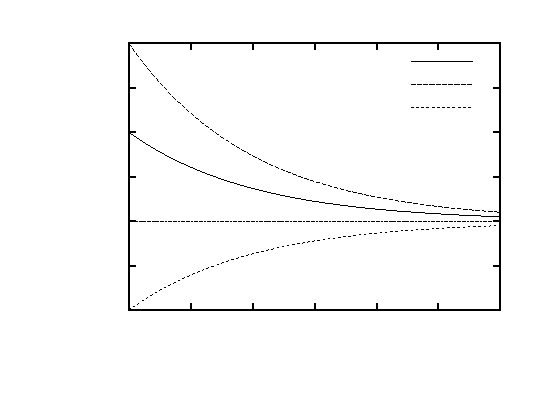
\includegraphics{bucket_v}}%
    \gplfronttext
  \end{picture}%
\endgroup

\end{center}
    }
\caption{Exponential relaxation. The dynamics described by the
  \lq{}bucket equation\rq{} is very common. Here
  $h(t)$ is plotted with
  $i=G$, $\tau=1$ and three different values of
  $h(0)$. $h(t)$ relaxes towards the equilibrium value, the closer it gets, the slower it approaches.\label{bucket_v}}
\end{figure}

\subsection*{Variable input}

We have only discussed constant inputs; the variable input case where
$i$ depends on time is harder and although it can sometimes be solved
it is often easier just to compute it numerically, we will look
briefly at how to do this, but first note that the effect of variable
inputis that the solution kind of chases the input with a timescale
set by $\tau$, that is for very small $\tau$ is chases it quickly, so
it is close to the input, but for large $\tau$ it lags behind it and
smooths it out. This is sometimes described by saying that it
\textsl{filters} the inout. There is an illustration in
Fig.~\ref{chasing}.

\begin{figure}

  \ifthenelse{\boolean{nopics}}{
    \textsl{In this graph the vertical axis runs from -1 to one, the horizonal from zero to 20. There is a sine wave marked input and three other curves, marked $\tau=0.25$, $\tau=2$ and $\tau=4$. The first of these is almost identical to the input curve, the other two are smoother and delayed with there peaks coming after the peaks of input, the peak for $\tau=2$ is around 0.55 and for $\tau=0.4$ it is around 0.3.}
  }
{\begin{center} % GNUPLOT: LaTeX picture with Postscript
\begingroup
  \makeatletter
  \providecommand\color[2][]{%
    \GenericError{(gnuplot) \space\space\space\@spaces}{%
      Package color not loaded in conjunction with
      terminal option `colourtext'%
    }{See the gnuplot documentation for explanation.%
    }{Either use 'blacktext' in gnuplot or load the package
      color.sty in LaTeX.}%
    \renewcommand\color[2][]{}%
  }%
  \providecommand\includegraphics[2][]{%
    \GenericError{(gnuplot) \space\space\space\@spaces}{%
      Package graphicx or graphics not loaded%
    }{See the gnuplot documentation for explanation.%
    }{The gnuplot epslatex terminal needs graphicx.sty or graphics.sty.}%
    \renewcommand\includegraphics[2][]{}%
  }%
  \providecommand\rotatebox[2]{#2}%
  \@ifundefined{ifGPcolor}{%
    \newif\ifGPcolor
    \GPcolorfalse
  }{}%
  \@ifundefined{ifGPblacktext}{%
    \newif\ifGPblacktext
    \GPblacktexttrue
  }{}%
  % define a \g@addto@macro without @ in the name:
  \let\gplgaddtomacro\g@addto@macro
  % define empty templates for all commands taking text:
  \gdef\gplbacktext{}%
  \gdef\gplfronttext{}%
  \makeatother
  \ifGPblacktext
    % no textcolor at all
    \def\colorrgb#1{}%
    \def\colorgray#1{}%
  \else
    % gray or color?
    \ifGPcolor
      \def\colorrgb#1{\color[rgb]{#1}}%
      \def\colorgray#1{\color[gray]{#1}}%
      \expandafter\def\csname LTw\endcsname{\color{white}}%
      \expandafter\def\csname LTb\endcsname{\color{black}}%
      \expandafter\def\csname LTa\endcsname{\color{black}}%
      \expandafter\def\csname LT0\endcsname{\color[rgb]{1,0,0}}%
      \expandafter\def\csname LT1\endcsname{\color[rgb]{0,1,0}}%
      \expandafter\def\csname LT2\endcsname{\color[rgb]{0,0,1}}%
      \expandafter\def\csname LT3\endcsname{\color[rgb]{1,0,1}}%
      \expandafter\def\csname LT4\endcsname{\color[rgb]{0,1,1}}%
      \expandafter\def\csname LT5\endcsname{\color[rgb]{1,1,0}}%
      \expandafter\def\csname LT6\endcsname{\color[rgb]{0,0,0}}%
      \expandafter\def\csname LT7\endcsname{\color[rgb]{1,0.3,0}}%
      \expandafter\def\csname LT8\endcsname{\color[rgb]{0.5,0.5,0.5}}%
    \else
      % gray
      \def\colorrgb#1{\color{black}}%
      \def\colorgray#1{\color[gray]{#1}}%
      \expandafter\def\csname LTw\endcsname{\color{white}}%
      \expandafter\def\csname LTb\endcsname{\color{black}}%
      \expandafter\def\csname LTa\endcsname{\color{black}}%
      \expandafter\def\csname LT0\endcsname{\color{black}}%
      \expandafter\def\csname LT1\endcsname{\color{black}}%
      \expandafter\def\csname LT2\endcsname{\color{black}}%
      \expandafter\def\csname LT3\endcsname{\color{black}}%
      \expandafter\def\csname LT4\endcsname{\color{black}}%
      \expandafter\def\csname LT5\endcsname{\color{black}}%
      \expandafter\def\csname LT6\endcsname{\color{black}}%
      \expandafter\def\csname LT7\endcsname{\color{black}}%
      \expandafter\def\csname LT8\endcsname{\color{black}}%
    \fi
  \fi
  \setlength{\unitlength}{0.0500bp}%
  \begin{picture}(7200.00,5040.00)%
    \gplgaddtomacro\gplbacktext{%
      \csname LTb\endcsname%
      \put(726,440){\makebox(0,0)[r]{\strut{}-1}}%
      \put(726,873){\makebox(0,0)[r]{\strut{}-0.8}}%
      \put(726,1307){\makebox(0,0)[r]{\strut{}-0.6}}%
      \put(726,1740){\makebox(0,0)[r]{\strut{}-0.4}}%
      \put(726,2174){\makebox(0,0)[r]{\strut{}-0.2}}%
      \put(726,2608){\makebox(0,0)[r]{\strut{} 0}}%
      \put(726,3041){\makebox(0,0)[r]{\strut{} 0.2}}%
      \put(726,3475){\makebox(0,0)[r]{\strut{} 0.4}}%
      \put(726,3908){\makebox(0,0)[r]{\strut{} 0.6}}%
      \put(726,4342){\makebox(0,0)[r]{\strut{} 0.8}}%
      \put(726,4775){\makebox(0,0)[r]{\strut{} 1}}%
      \put(858,220){\makebox(0,0){\strut{} 0}}%
      \put(1453,220){\makebox(0,0){\strut{} 2}}%
      \put(2047,220){\makebox(0,0){\strut{} 4}}%
      \put(2642,220){\makebox(0,0){\strut{} 6}}%
      \put(3236,220){\makebox(0,0){\strut{} 8}}%
      \put(3831,220){\makebox(0,0){\strut{} 10}}%
      \put(4425,220){\makebox(0,0){\strut{} 12}}%
      \put(5020,220){\makebox(0,0){\strut{} 14}}%
      \put(5614,220){\makebox(0,0){\strut{} 16}}%
      \put(6209,220){\makebox(0,0){\strut{} 18}}%
      \put(6803,220){\makebox(0,0){\strut{} 20}}%
    }%
    \gplgaddtomacro\gplfronttext{%
      \csname LTb\endcsname%
      \put(5816,4602){\makebox(0,0)[r]{\strut{}$\tau=0.25$}}%
      \csname LTb\endcsname%
      \put(5816,4382){\makebox(0,0)[r]{\strut{}$\tau=2$}}%
      \csname LTb\endcsname%
      \put(5816,4162){\makebox(0,0)[r]{\strut{}$\tau=4$}}%
      \csname LTb\endcsname%
      \put(5816,3942){\makebox(0,0)[r]{\strut{}input}}%
    }%
    \gplbacktext
    \put(0,0){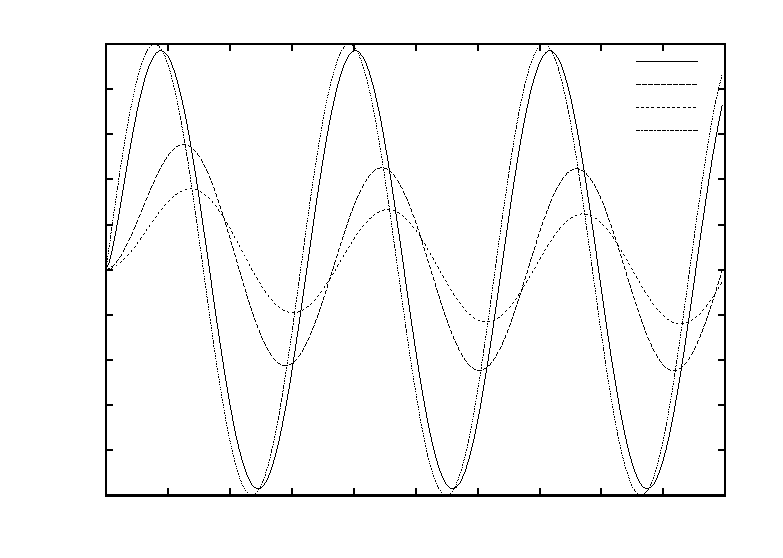
\includegraphics{chasing}}%
    \gplfronttext
  \end{picture}%
\endgroup
\end{center}}
\caption{Variable input. Here the input is a sine wave $i(t)=\sin{t}$
  and the equation is evolved with $h(0)=0$ and three different $\tau$
  values. For $\tau=0.25$ we see $h(t)$ closely matches the input
  whereas for larger $\tau$ it is smoother and lags
  behind.\label{chasing}}
\end{figure}


\subsection*{Numerical solutions}

Consider the problem of solving a general first order differential equation
\begin{equation}
\frac{df(t)}{dt}=F(f,t)
\end{equation}
This includes our bucket case if we replace $f$ with $h$ and $F(f,t)$
with $(i-Gh)/C$. Now consider the situation where we want to solve
this but can't do it analytically, as will be the case for many
values of the time dependent input $i(t)$ or, indeed, if $i(t)$ itself
is only known numerically. 

The simplest numerical approach is Euler's method. Say you know the value of $f(t)$ and want to approximate $f(t+\delta t)$ where $\delta t$ is some small increment in time. Now, it is known that
\begin{equation}
f(t+\delta t)=f(t)+\delta t \frac{df(t)}{dt}+O(\delta t^2)
\end{equation}
That is, it changes by its rate of change multiplied by how long it is
changing for. The $O(\delta t^2)$ says there are $\delta t^2$ sized
errors in this approximation, this comes about because $dh/dt$ is
itself changing but our approximation assumes it is fixed still. Now we
know what $df(t)/dt$ is, it is $F(f,t)$ from the equation, so
\begin{equation}
f(t+\delta t)=f(t)+\delta t F(f,t) + O(\delta t^2)
\end{equation}
so approximating $f(t+\delta t)$ with $f(t)+\delta t F(f,t)$ is actual
to first order in the time step $\delta t$. This is the Euler
approximation. More formally if we have an initial condition $f(t_0)$ and write
\begin{align}
f_n&=f(t_0+n\delta t)\\
t_n&=t_0+n\delta t
\end{align}
then the Euler approximation is
\begin{equation}
f_{n+1}=f_n+\delta t F(f_n,t_n)
\end{equation}
Thus, in the case we are interested in here
\begin{equation}
h_{n+1}=\frac{[i(t_n)-Gh_n]\delta t}{C}
\end{equation}

Of course, this is just the easiest way to do the integration, there
are more sophisticated approaches like Runge-Kutta or backwards Euler
which are more complex and computational costly for each step, but
which are also much more accurate.

\section{Summary}

Water filling a leaky bucket gives a useful example of the dynamics that will describe a neuron. The idea is that the leak is proportional to the height of the water, so we write:
\begin{equation}
  l(t)=Gh(t)
\end{equation}
The volume of water is also proportional to the height, so we write:
\begin{equation}
  \text{vol}=Ch(t)
\end{equation}
where $G$ and $C$ are both constants of proportionality, the $G$ will
depend in a complicated way on the viscosity of water, the size of the
hole, the $C$ is more straight-forwardly the cross-sectional area of
the bucket. Given that the rate of change of volume is given by water
coming in minus water going out, an writing $i(t)$ for the inflow:
\begin{equation}
\frac{dCh(t)}{dt}=i(t)-Gh(t)
\end{equation}
This can also be written
\begin{equation}
\tau\frac{dh}{dt}=Ri-h
\end{equation}
where $R=1/G$ and $\tau=C/G$ is a timescale. By solving for constant
input and discussing the dynamics we see that the solution to this
equation `chases' the input $Ri$ over a timescale corresponding to
$\tau$. Finally we look at numerical approaches: for the Euler
approximation, the approximate solution at a time $t_n=n\delta t$ is
\begin{equation}
  h_n=h_{n-1}+\delta t \left.\frac{dh}{dt}\right|_{t_n}
\end{equation}

\end{document}

